\documentclass[13.5pt,aspecratio=169, xcolor=dvipsnames]{beamer}
\usepackage{graphicx} % Required for inserting images
\usepackage{subcaption}
\usepackage{amsfonts}
\usepackage{amsmath}
\usepackage{amssymb}
\usepackage{physics}
\usepackage{bm}
\usepackage{physics}
\usepackage{booktabs}
\usepackage{setspace}
\usepackage{xcolor}
\usepackage{wrapfig,lipsum}
\usepackage{etoolbox}
\usepackage{tikz}
\usepackage[most]{tcolorbox}
\usetheme{Madrid}
\useinnertheme{circles}

\DeclareMathOperator*{\argmax}{arg\,max}
\DeclareMathOperator*{\argmin}{arg\,min}
\graphicspath{{Images/}{./}} 
\usetheme{Copenhagen}
\definecolor{UBCblue}{rgb}{0.04706, 0.13725, 0.26667} 
\usecolortheme[named=UBCblue]{structure}
%\usecolortheme{beaver}
% \titlegraphic{\centering \LARGE MultiVerS}
\title{Improving scientific claim verification with
weak supervision and full-document context}
\author[CS221]{
    \begin{tabular}{c}
        \textbf{CS221.O12.KHCL} \\
        \textit{Instructor: PhD. Nguyen Thi Quy} \\
        \bigskip
        \textbf{Group 15} \\
        Le Gia Khang \quad Nguyen Hoang Tan \quad Le Duy Khang
    \end{tabular}
}
\date{\today}
\definecolor{mylightgreencolor}{RGB}{144, 238, 144}
\definecolor{mylightredcolor}{RGB}{255, 204, 203}
\definecolor{mylightbluecolor}{RGB}{173,216,230}
\setbeamertemplate{navigation symbols}{}
\setbeamertemplate{headline}{}
\setbeamercolor{huge text}{fg=white}
\setbeamertemplate{footline}{
    \leavevmode%
    \hbox{%
        \begin{beamercolorbox}[wd=.2\paperwidth,ht=2.25ex,dp=1ex,center]{author in head/foot}%
            \usebeamerfont{author in head/foot}\insertshortauthor
        \end{beamercolorbox}%
        \begin{beamercolorbox}[wd=.6\paperwidth,ht=2.25ex,dp=1ex,center]{title in head/foot}%
            \usebeamerfont{title in head/foot}\insertshorttitle
        \end{beamercolorbox}%
        \begin{beamercolorbox}[wd=.2\paperwidth,ht=2.25ex,dp=1ex,right]{date in head/foot}%
            \insertframenumber{} / \inserttotalframenumber\hspace*{2ex} 
        \end{beamercolorbox}%
    }%
    \vskip0pt%
}
\setbeamertemplate{section in toc}{%
  \tikz[baseline=(tocseclabel.base)]{
    \node[fill=structure.fg,rounded corners,inner sep=4pt, font=\large\bfseries] (tocseclabel) {\color{white}\inserttocsectionnumber};
  }\hspace{0.5em}\large\bfseries\inserttocsection\vspace{0.3em}}

  
\begin{document}
\begin{frame}
    \begin{picture}(0,0)
        \put(170,0){\makebox(0,0){\huge \textbf{\textcolor{UBCblue}{MultiVerS}}}}
    \end{picture}
    \maketitle
\end{frame}

% \begin{frame}
% 	\frametitle{Table of Contents} % Slide title, remove this command for no title
% 	\tableofcontents[subsectionstyle=hide]
% \end{frame}
%-------------------------------------------------------------------%


% \begin{frame}
%     \doublespacing
%         \frametitle{Presentation Overview} % Slide title, remove this command for no title
        
%         \tableofcontents % Output the table of contents (all sections on one slide)
%         %\tableofcontents[pausesections] % Output the table of contents (break sections up across separate slides)
% \end{frame}
    
%     %----------------------------------------------------------------------------------------
%     %	PRESENTATION BODY SLIDES
%     %----------------------------------------------------------------------------------------
    
%     \section{Lexical Semantics} % Sections are added in order to organize your presentation into discrete blocks, all sections and subsections are automatically output to the table of contents as an overview of the talk but NOT output in the presentation as separate slides
%     %------------------------------------------------
%     \begin{frame}
%         \doublespacing
%             \frametitle{Presentation Overview} % Slide title, remove this command for no title
            
%             \tableofcontents[currentsection] % Output the table of contents (all sections on one slide)
%             %\tableofcontents[pausesections] % Output the table of contents (break sections up across separate slides)
%     \end{frame}

% %-------------------------------------------------------------------%


\begin{frame}
    \onehalfspacing
    \frametitle{Task}
    \begin{minipage}{0.47\textwidth}
        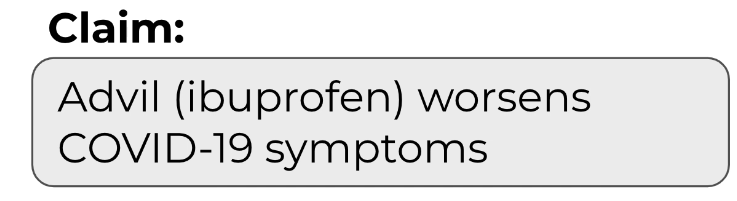
\includegraphics[width=\textwidth]{Claim.png}
        \visible<2-5> {
            \centering
            \begin{minipage}{0.7\textwidth}
            {\setbeamercolor{block body}{bg=Maroon}
            \begin{block}{}
                \begin{center}
                    \textbf{\textcolor{white}{Label: Refuted}}
                \end{center}
            \end{block}
            }
            \end{minipage}     
        }
        
        \bigskip
        \visible<3-5> {
            \begin{flushleft}
            Task Outputs
            \begin{enumerate}
                \item Fact-checking label
                \visible<4-> {\item Rationales justifying the label}
            \end{enumerate}
            \end{flushleft}
        }

    \end{minipage}
    \begin{minipage}{0.45\textwidth}
        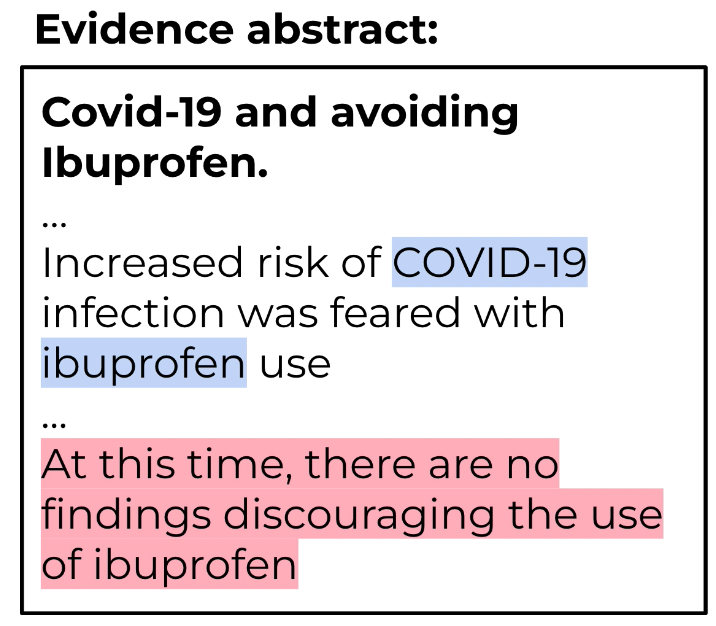
\includegraphics[width=1.2\textwidth]{Evidence_abstract.png}
        
        \visible<4-5> {
            \setbeamercolor{block body}{bg=mylightredcolor}
            \vspace*{-2.5em}
            \hspace{9em}
            \begin{minipage}{0.4\textwidth}
            \begin{block}{}
                \begin{center}
                    \textbf{\textcolor{black}{Rationale}}
                \end{center}
            \end{block}
         \end{minipage}     
        }

        \visible<5> {
            \setbeamercolor{block body}{bg=mylightbluecolor}
            \vspace*{-8em}
            \hspace{9em}
            \begin{minipage}{0.5\textwidth}
            \begin{block}{}
                \begin{center}
                    {\textcolor{black}{Context required}}
                \end{center}
            \end{block}
         \end{minipage}     
        }
    \end{minipage}
\end{frame}
    
%--------------------------------------------------

    \begin{frame}
    \onehalfspacing
        \frametitle{Prior work: Extract-then-label}
        \only <1> {
            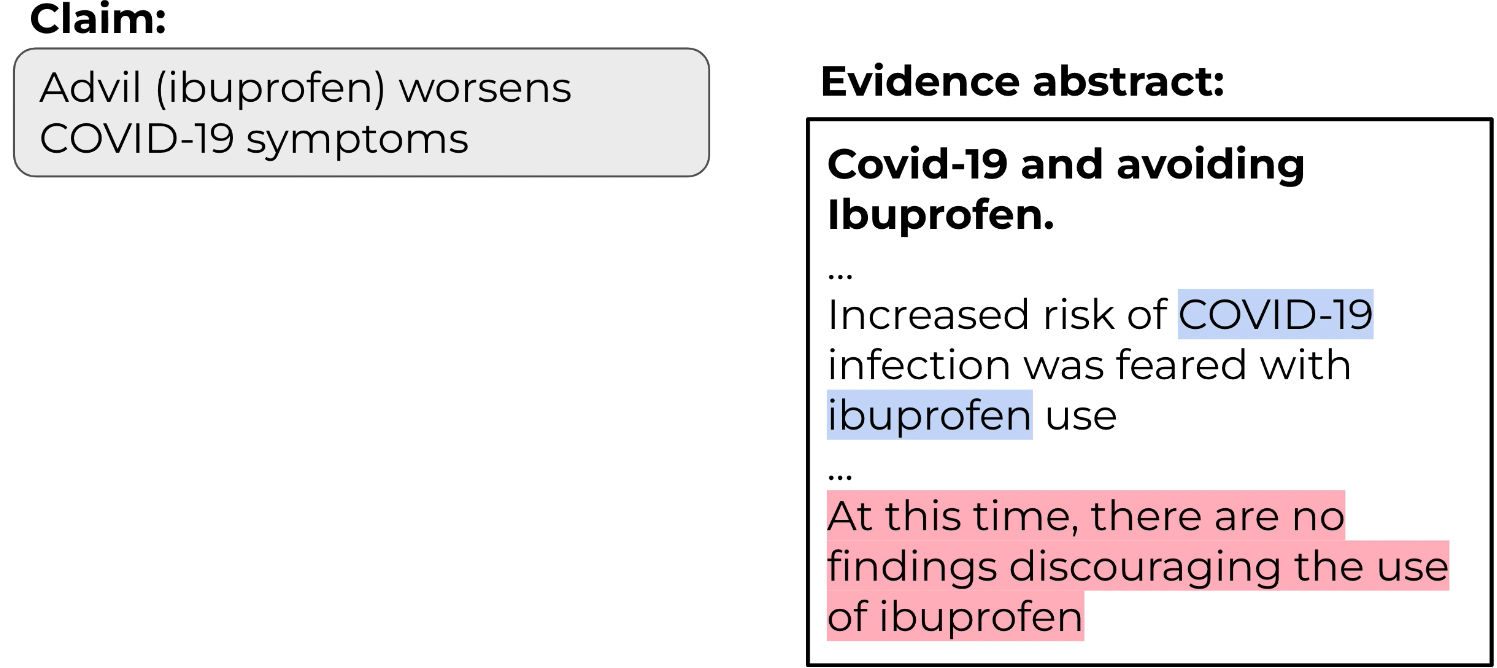
\includegraphics[width=\textwidth]{Extract_then_label_1.png}
        }
        \only <2-> {
            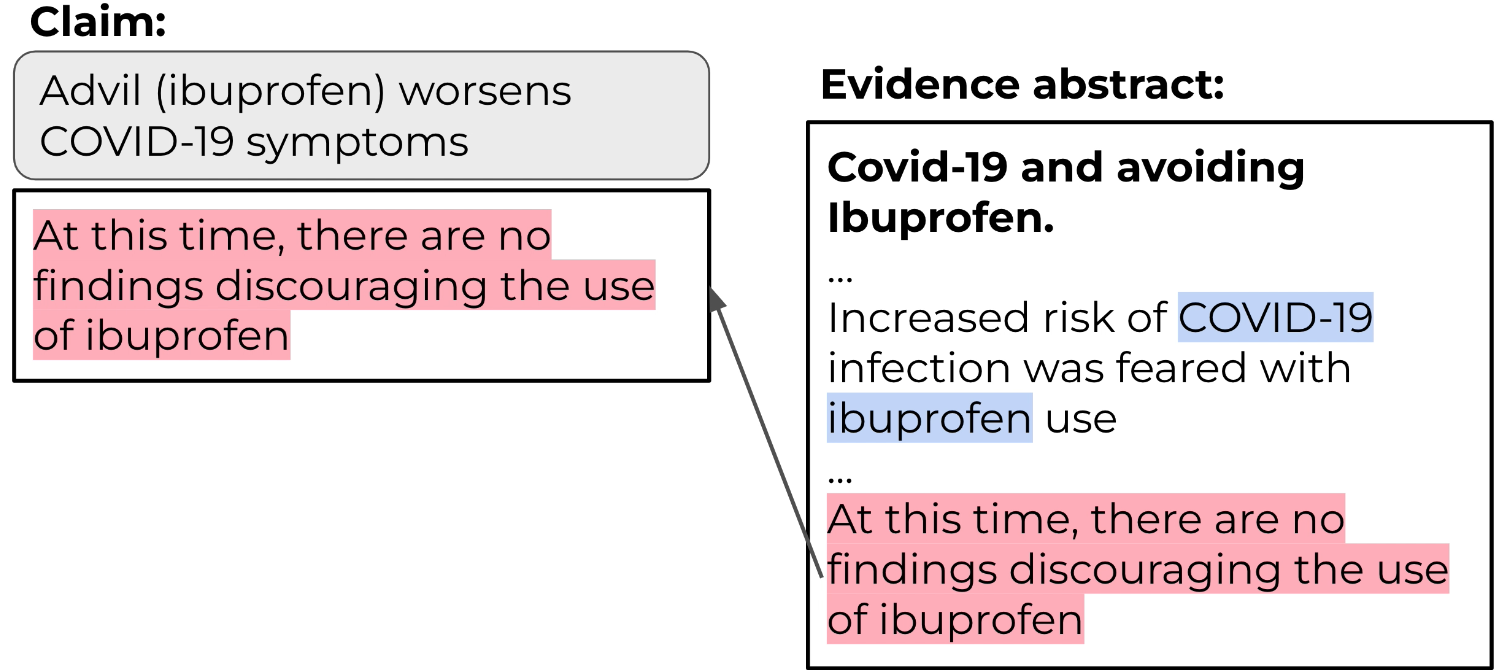
\includegraphics[width=\textwidth]{Extract_then_label_2.png}
        }

        \only <3-> {
            \vspace*{-7em}
            
\includegraphics[width=0.5\textwidth]{produce_label.png}
        }

        \only <4> {
            \begin{overlayarea}{\textwidth}{\textheight}
                \vspace*{-3.5em}
                \hspace*{17em}
                \begin{minipage}{0.45\textwidth}
                    \begin{block}{Drawbacks of extract-then-label:}
                        \begin{enumerate}
                            \item Rationales may lack context
                            \item Requires rationale supervision during training
                        \end{enumerate}
                    \end{block}
                \end{minipage}
            \end{overlayarea}
        }
    \end{frame}
    
    
    %------------------------------------------------
    \begin{frame}
        \onehalfspacing
            \frametitle{MultiVerS}
            \only<1>{
                \begin{figure}[h]
                    \centering
                    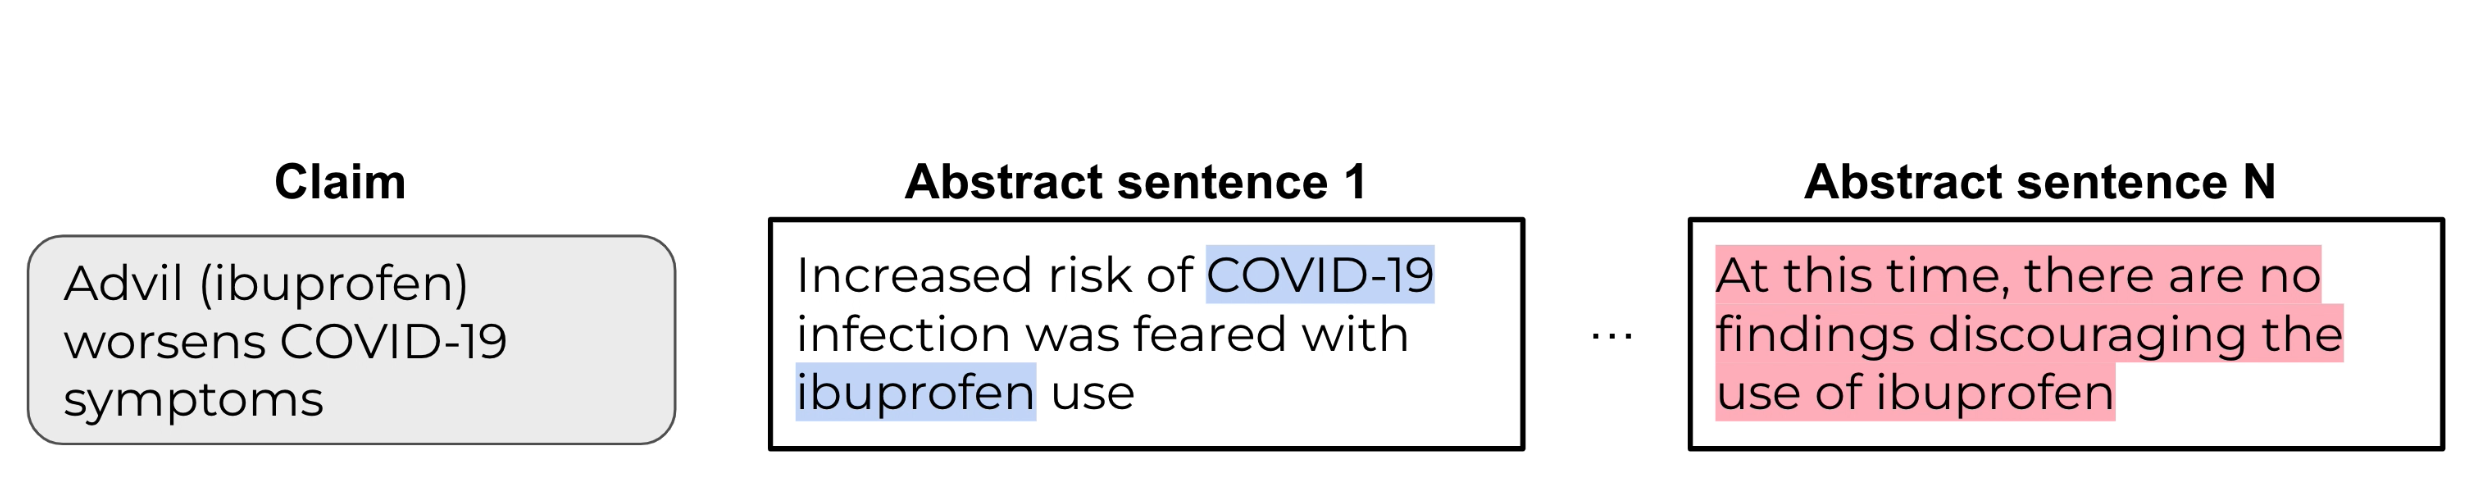
\includegraphics[width=\linewidth]{MultiVerS_1.png}
            \end{figure}
            }
            \only<2>{
                \begin{figure}[h]
                    \centering
                    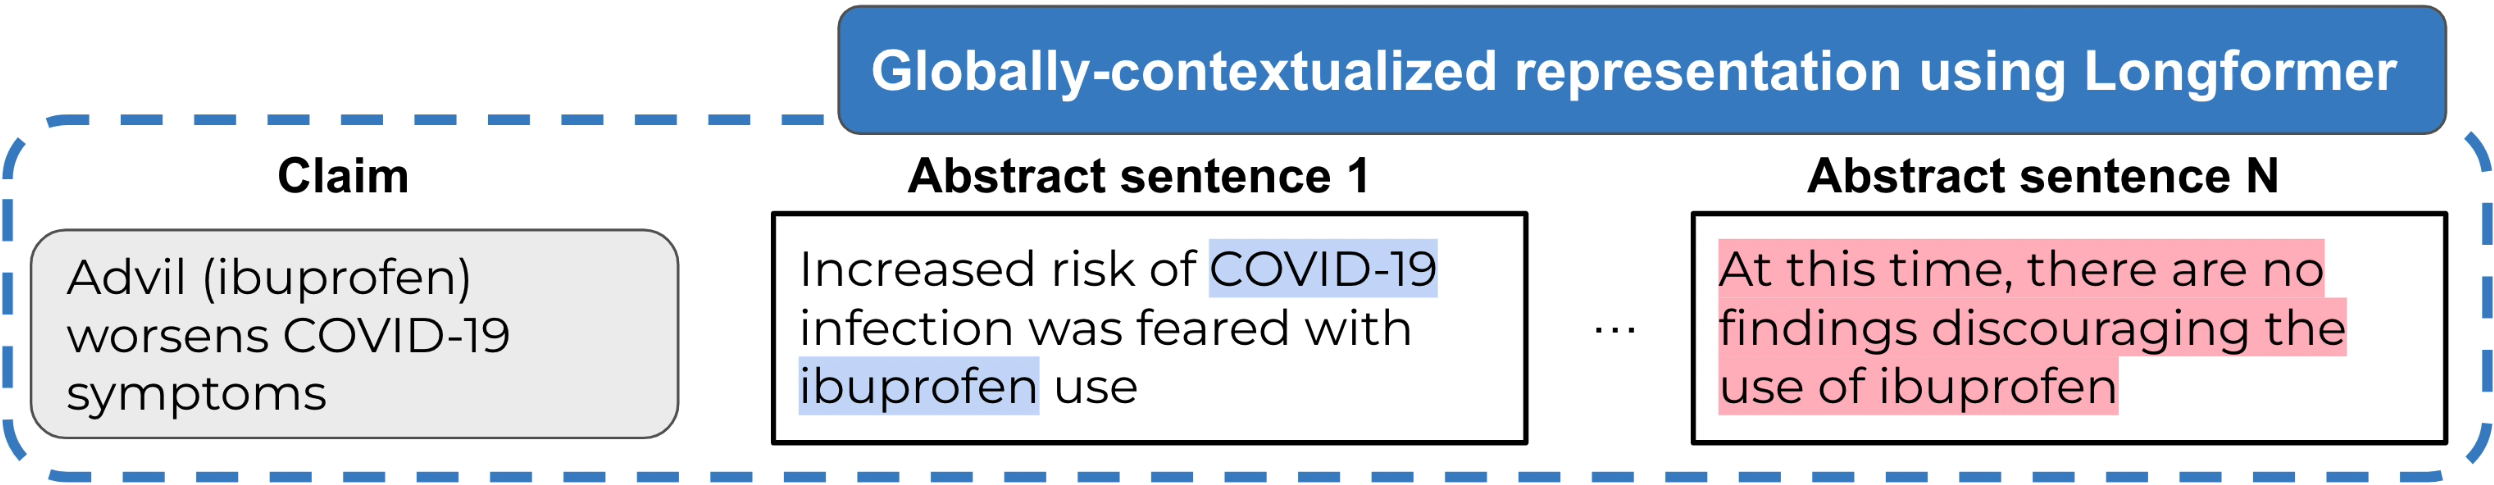
\includegraphics[width=\linewidth]{MultiVerS_2.png}
            \end{figure}
            }

            \only<3>{
                \begin{figure}[h]
                    \centering
                    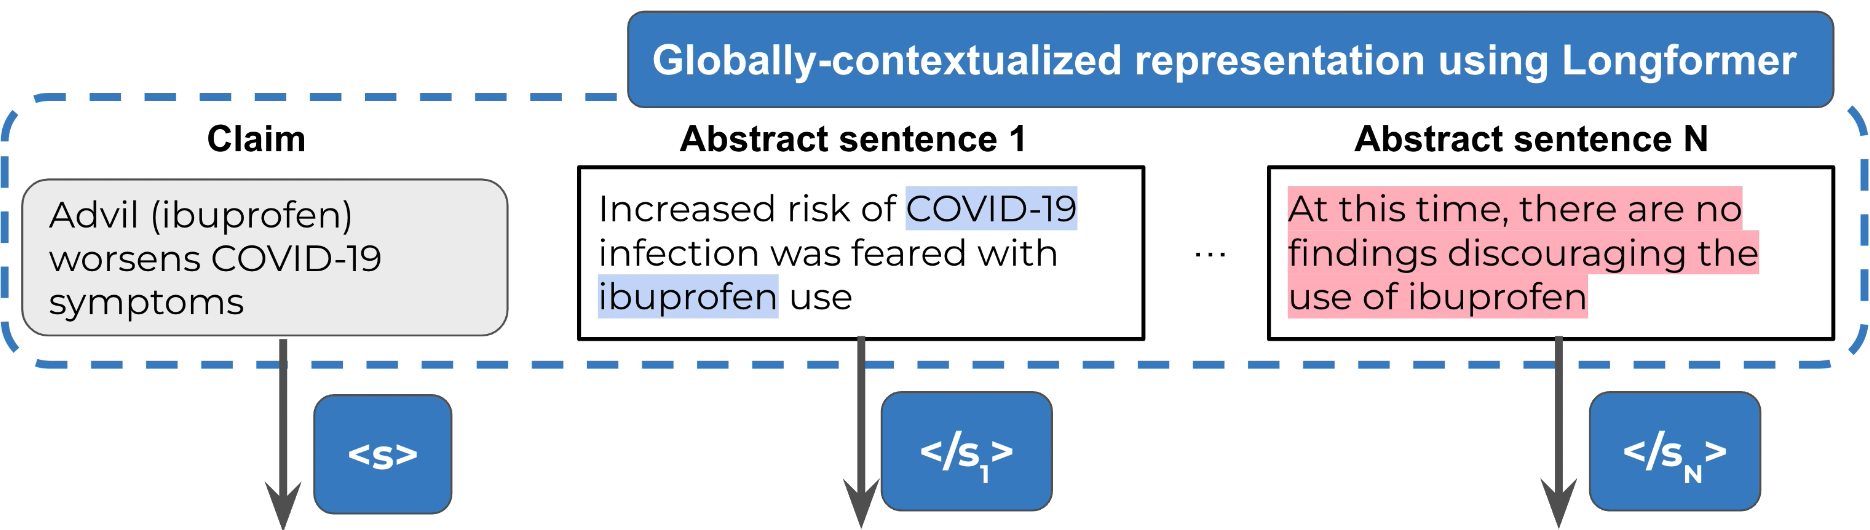
\includegraphics[width=\linewidth]{MultiVerS_3.png}
            \end{figure}
            }

            \only<4->{
                \begin{figure}[h]
                    \centering
                    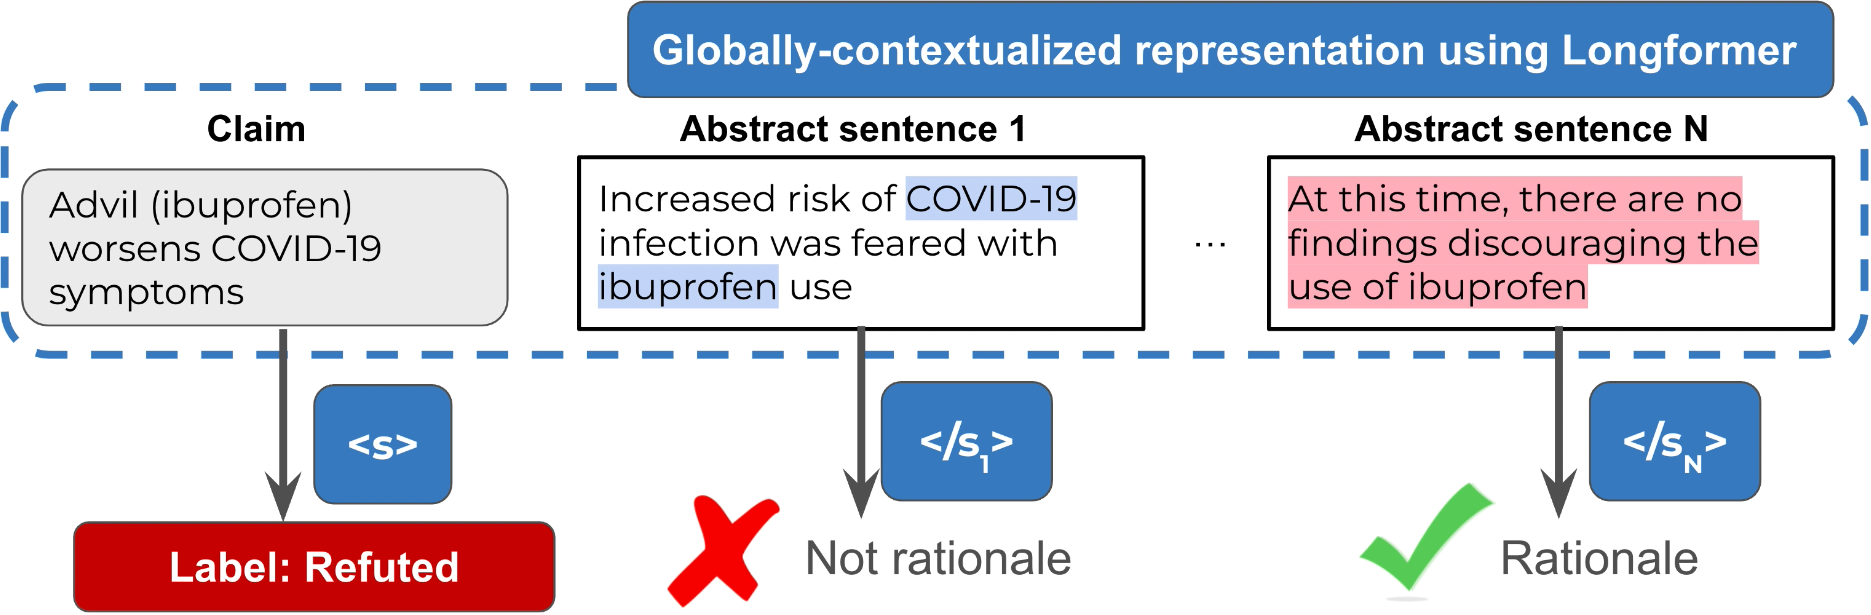
\includegraphics[width=\linewidth]{MultiVerS_4.png}
                \end{figure}
            }

            \only<5-> {
                 \begin{minipage}{0.52\textwidth}
                    {\Large
                    \begin{tcolorbox}[ams align,colback=white]
                        \hspace{-0.75em} \mathcal{L} = \mathcal{L}_{label} + \lambda_{rationale} \mathcal{L}_{rationale} \nonumber
                    \end{tcolorbox}
                    }
                \end{minipage}
                \hspace{0.2em}
                \begin{minipage}{0.45\textwidth}
                    \begin{block}{Benefits of multitask approach:}
                        \begin{enumerate}
                            \item Incorporates all relevant context
                            \item Can train on instances with no rationale annotations
                        \end{enumerate}
                    \end{block}
                \end{minipage}
            }
                
\end{frame}
    
%------------------------------------------------
    

\begin{frame}
\onehalfspacing
    \frametitle{Experiments}
    \begin{minipage}{0.3\textwidth}
        \textbf{Text datasets:}
        \begin{itemize}
            \item HealthVer
            \item COVID-Fact
            \item SciFact
        \end{itemize}
    \end{minipage}
    \begin{minipage}{0.69\textwidth}
        \visible <2-> {
        \begin{minipage}{0.75\textwidth}
            \begin{block}{}
                \hspace{0.5em} Roughly 1000 claims / dataset. \\
                \hspace{0.5em} Expert annotations are expensive
            \end{block}
        \end{minipage} 
        }
    \end{minipage}

    \bigskip
    \visible<3-> {
        \textbf{Traning procedure:}
        \begin{itemize}
            \item \textbf{Stage 1:} Train on a combination of \textit{labeled out of domain} data \textit{weekly-labeled in-domain data.}
            \item \textbf{Stage 2:} Continue training on data from each target dataset. 
        \end{itemize}
    }
    \bigskip
    \vspace*{-1em}
    \visible<4-> {
        \textbf{Domain adaptation settings:}
        \begin{itemize}
            \item \textbf{Zero-shot:} Stage 1 training only.
            \item \textbf{Few-shot:} 45 instances from target datasets.
            \item \textbf{Full-supervised:} All target data.
        \end{itemize}
    }



\end{frame}
%------------------------------------------------


\begin{frame}
    \onehalfspacing
        \frametitle{Data: Stage 1}
        \begin{minipage}[t]{0.42\textwidth}
            {
            \vspace*{-7em}
            \centering
            \textbf{Supervised} out-of-domain data (FEVER)

            

            \begin{block}{}
                LeBron James was born in \\ Ohio
            \end{block}
            {
            \setbeamercolor{block body}{bg=mylightgreencolor}

                \vspace*{-2em}
                \hspace{3em}
                \begin{minipage}{0.7\textwidth}

                \begin{block}{}
                    \centering
                    Label: Supported
                \end{block}
            \end{minipage}
            }

            \bigskip
            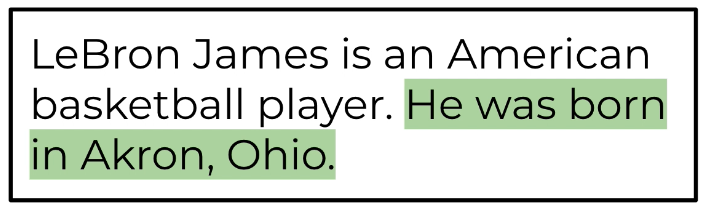
\includegraphics[width=\textwidth]{LeBron_James_claim.png}
            }
        \end{minipage}
        \hfill\vrule height 90pt width 2pt\hfill
        \begin{minipage}[t]{0.54\textwidth}
            {
            \vspace*{-7em}

            \only<1> {
                \phantom{
                \centering
                \textbf{Weekly-supervised} in-domain data
                fdjjnf
                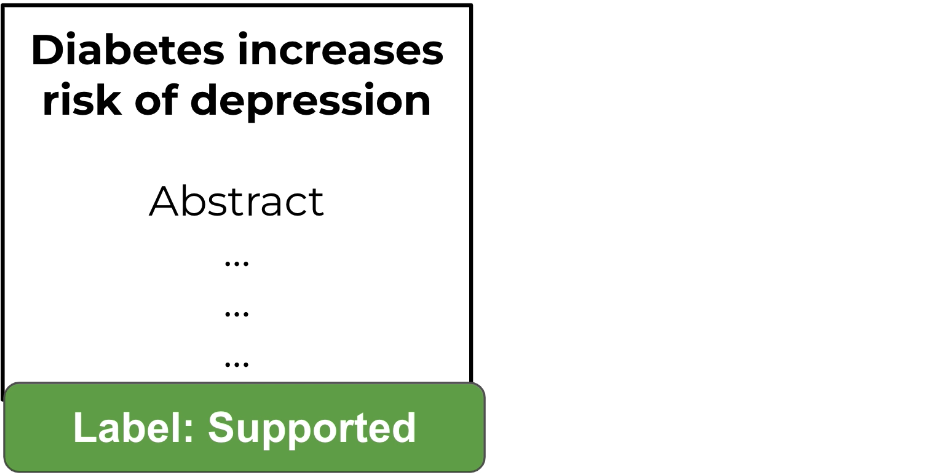
\includegraphics[width=\textwidth]{Stage_1_data_0.png} 
                }

            }

            \only<2-> {
                \centering
                \textbf{Weekly-supervised} in-domain data
                \phantom{                fdjjnf
                }
            }
            \only<2> {
                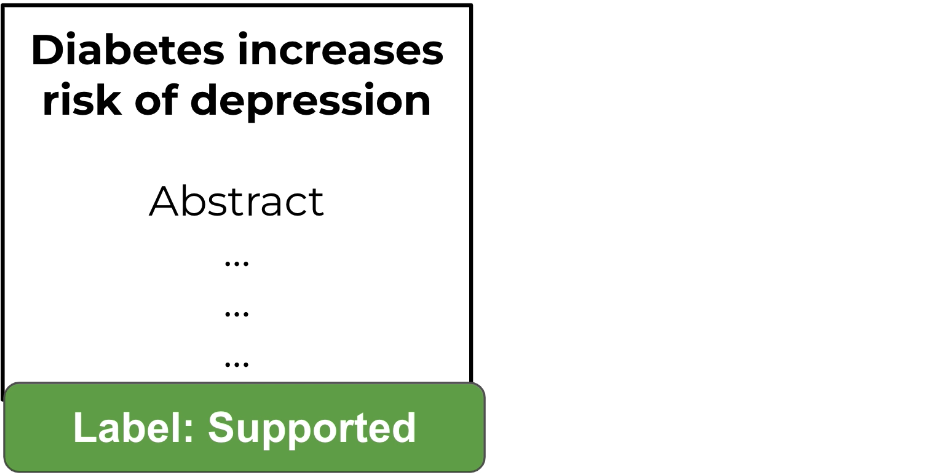
\includegraphics[width=\textwidth]{Stage_1_data_0.png}
            }

            \only<3> {
                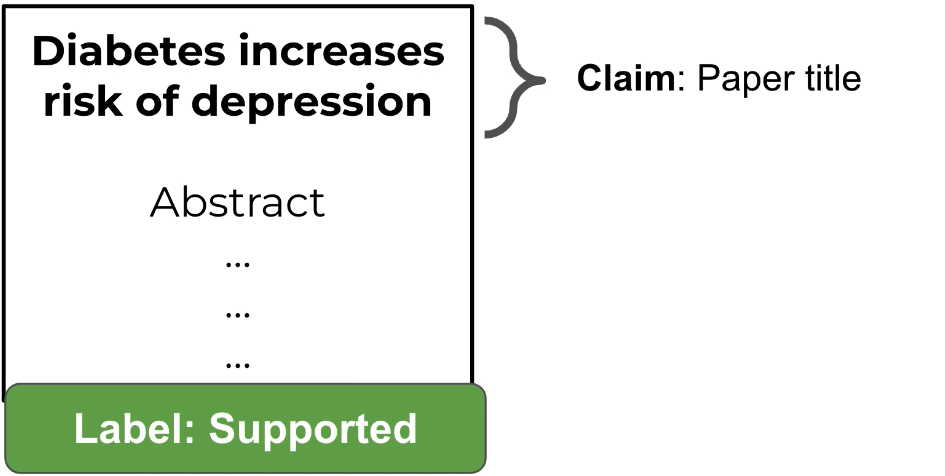
\includegraphics[width=\textwidth]{Stage_1_data_1.png}
            }

            \only<4-> {
                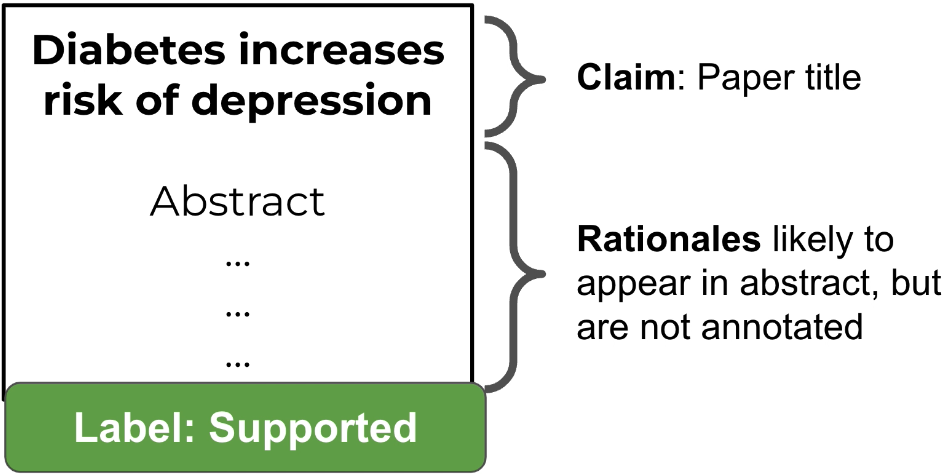
\includegraphics[width=\textwidth]{Stage_1_data_2.png}
            }

            \vspace*{-2em}
            \visible<5> {
                \begin{center}
                    \begin{minipage}{0.9\textwidth}
                        \begin{block}{}
                            MultiVerS can train on these examples, even though no rationale annotations are provided
                        \end{block}
                    \end{minipage}
                \end{center}
            }
            }
        \end{minipage}
       


    
    
\end{frame}
%------------------------------------------------


\begin{frame}
    \onehalfspacing
        \frametitle{Results}

        \only<1> {
            \vspace*{-2pt}
            \hspace{1pt}
            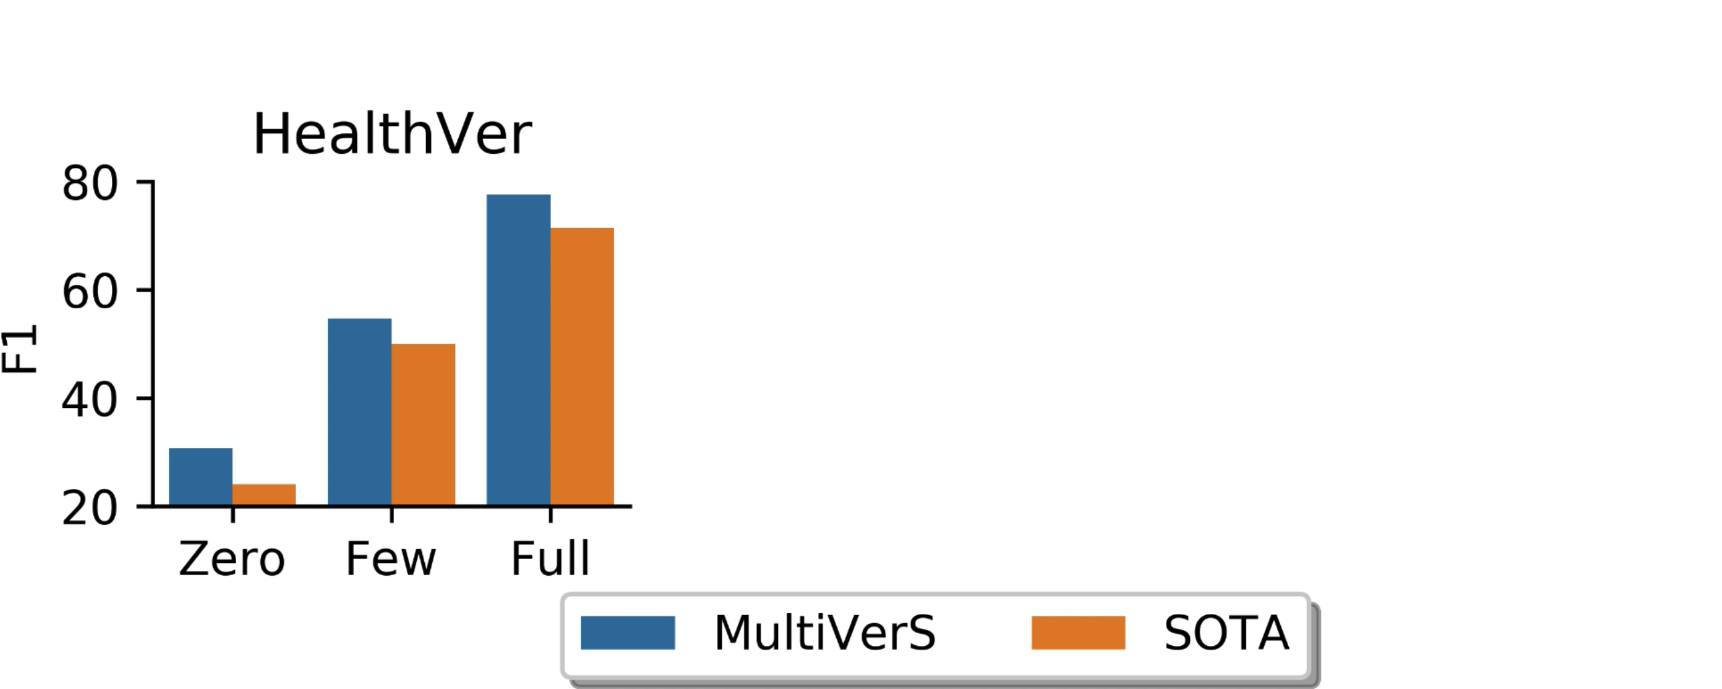
\includegraphics[width=\textwidth]{Result_0.png}

        }
        \only<2> {
            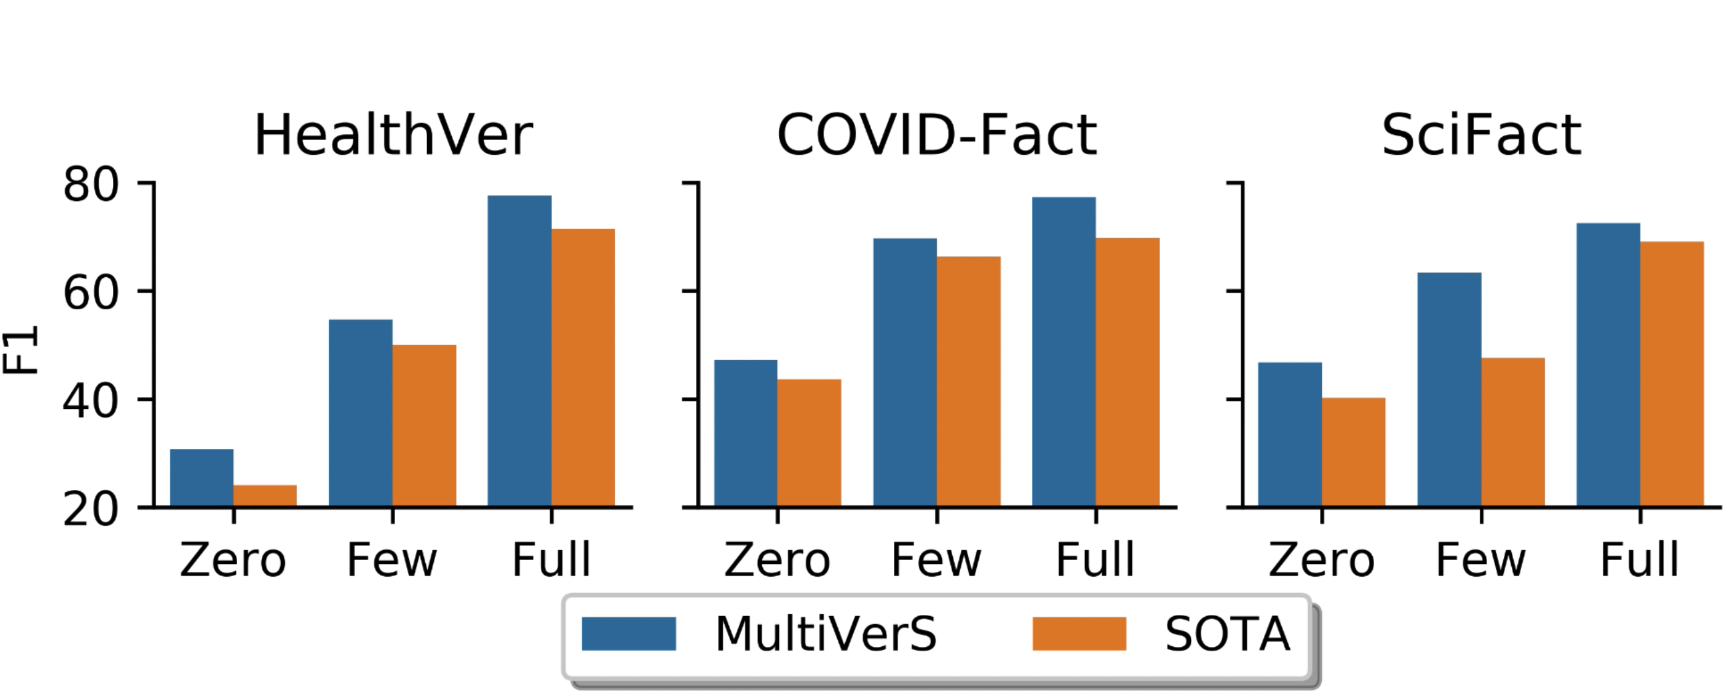
\includegraphics[width=\textwidth]{Result_1.png}

            \begin{minipage}{0.6\textwidth}
                \begin{block}{}
                    \vspace*{0.5em}MultiVerS outperforms SOTA on all datasets
                \end{block}
            \end{minipage}
        }
       

    
\end{frame}
%------------------------------------------------

\begin{frame}
    \onehalfspacing
        \frametitle{Results}

        \only<1> {
            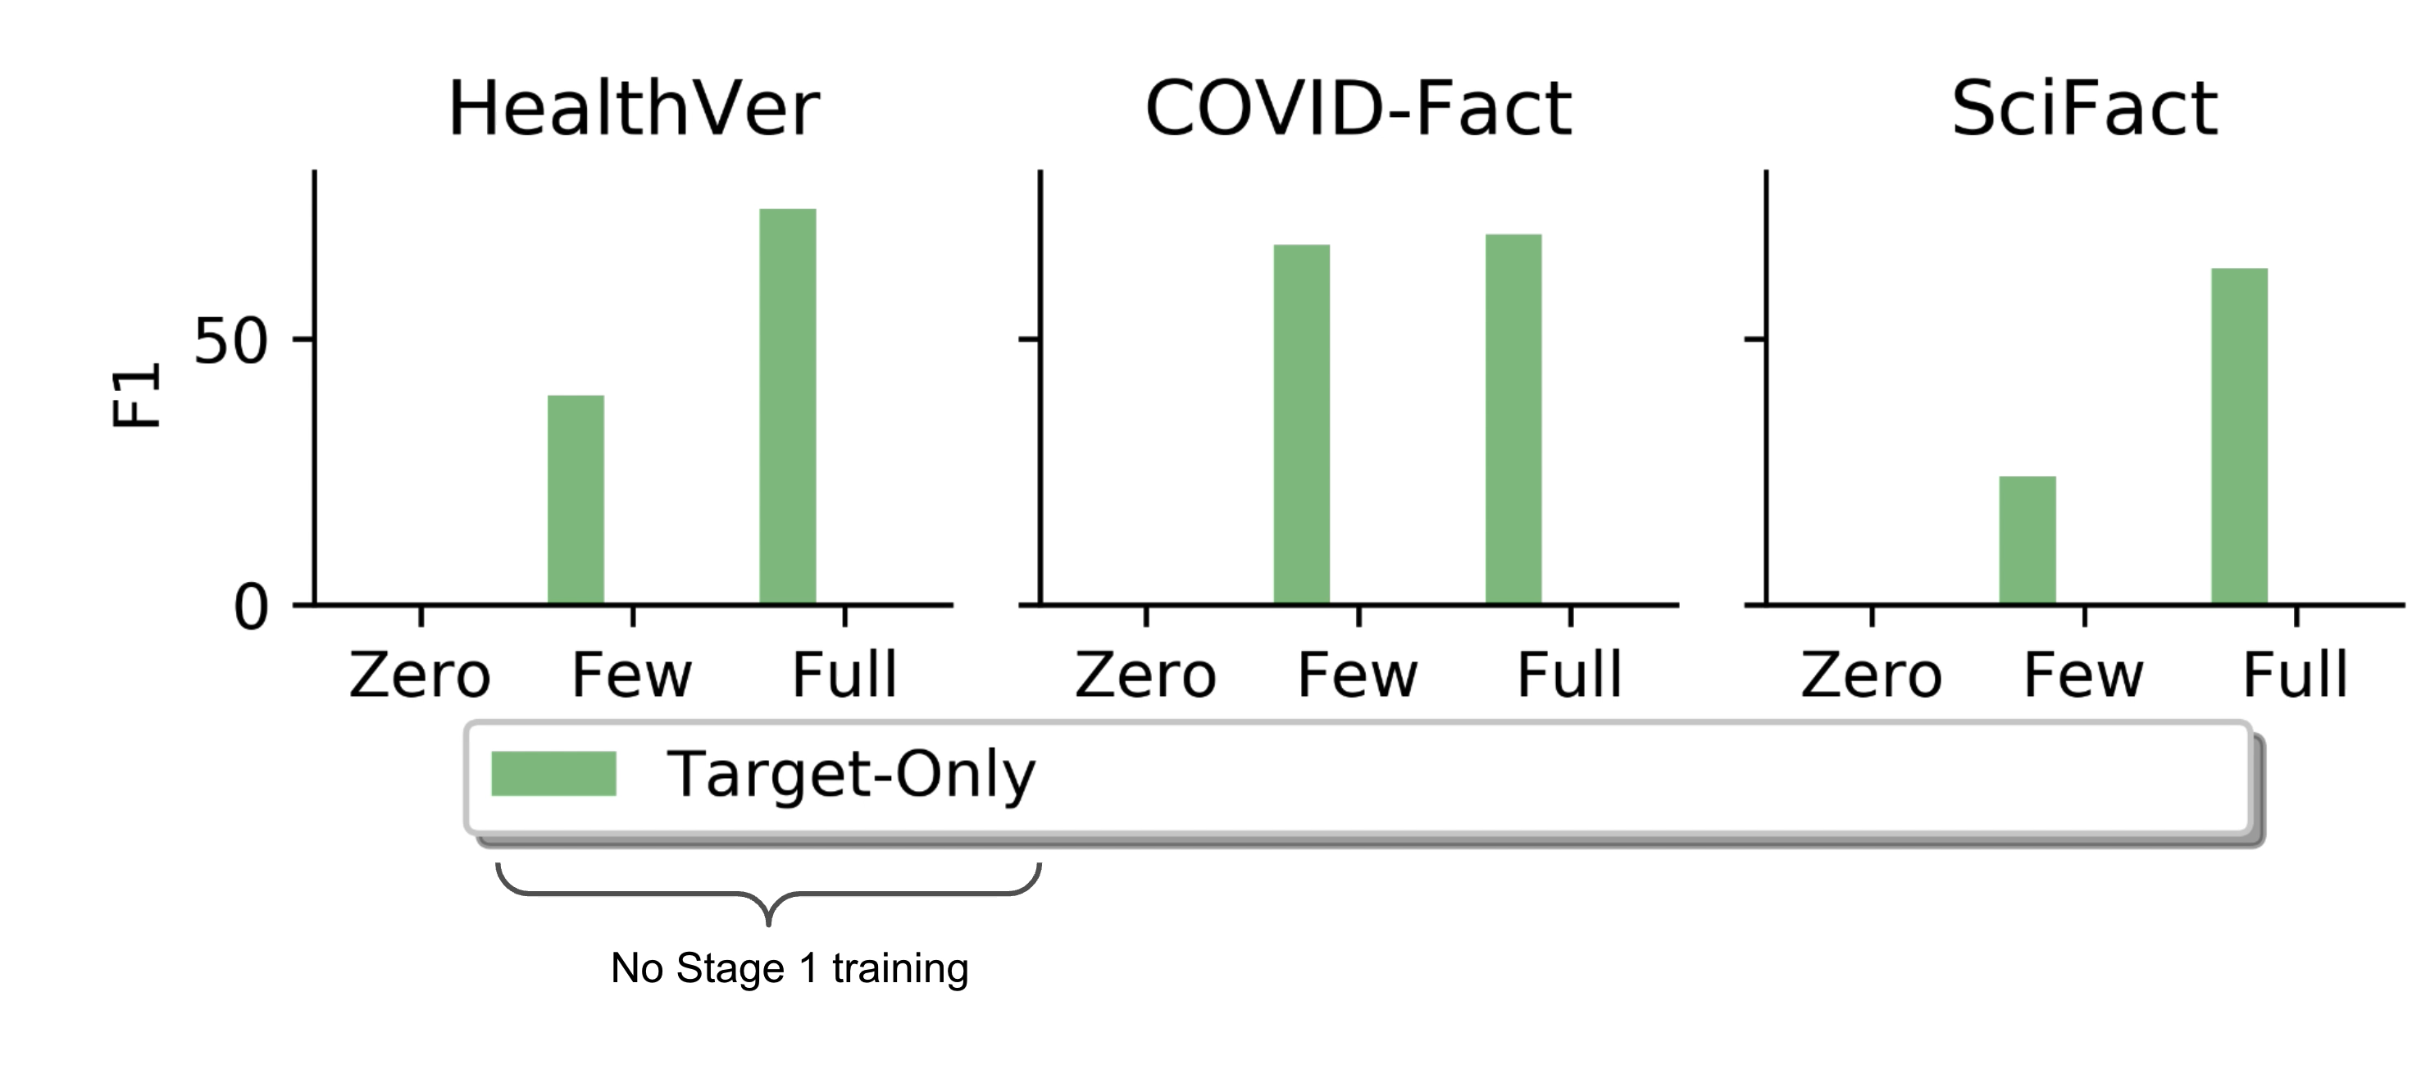
\includegraphics[width=1\textwidth]{Crop/Ablations_1.png}
        }
        \only<2> {
            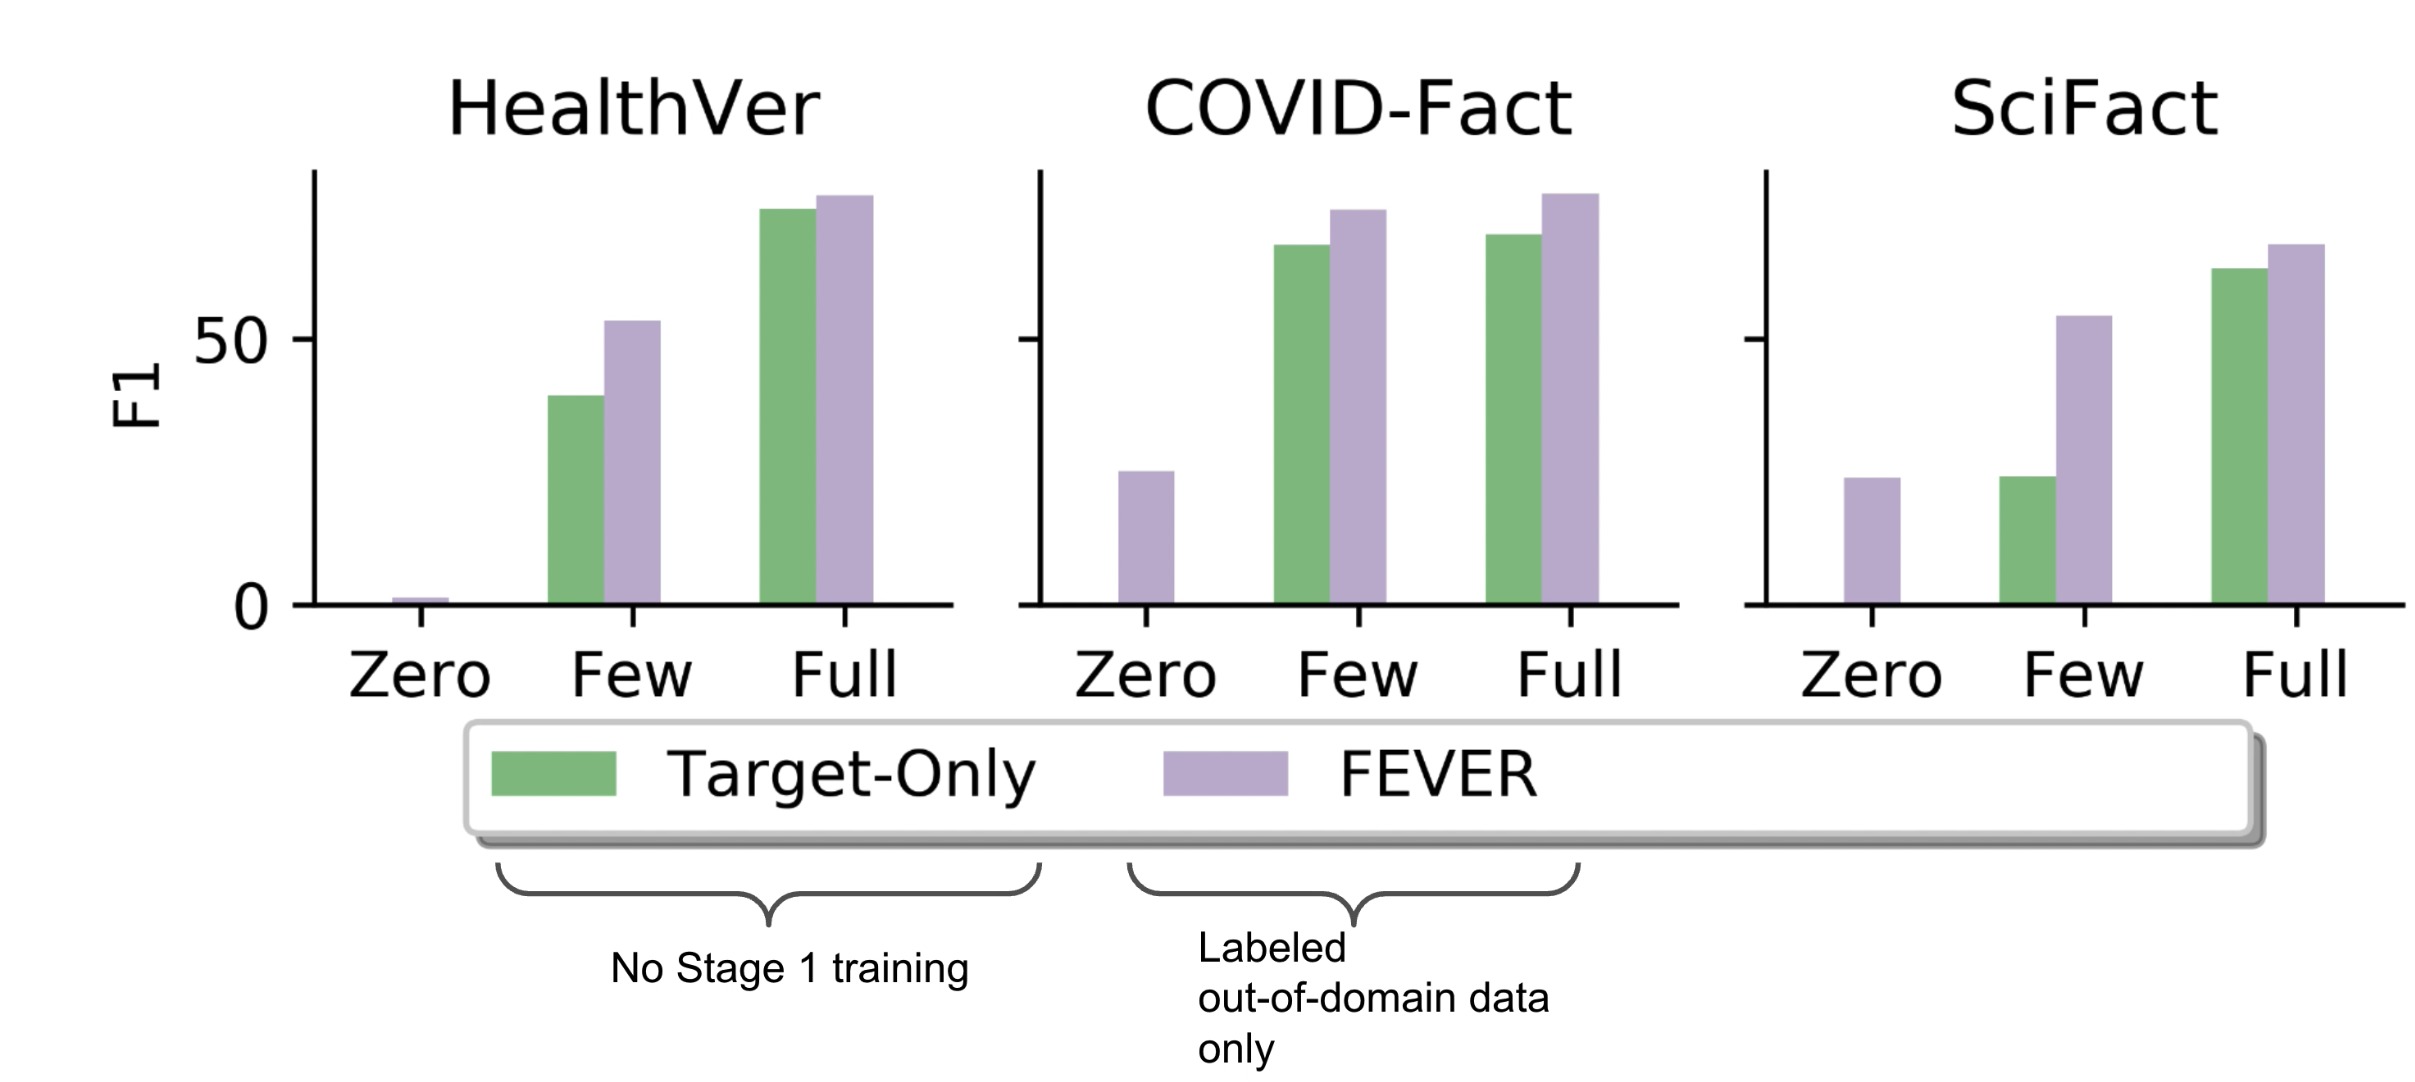
\includegraphics[width=1\textwidth]{Crop/Ablations_2.png}
        }
        \only<3-> {
            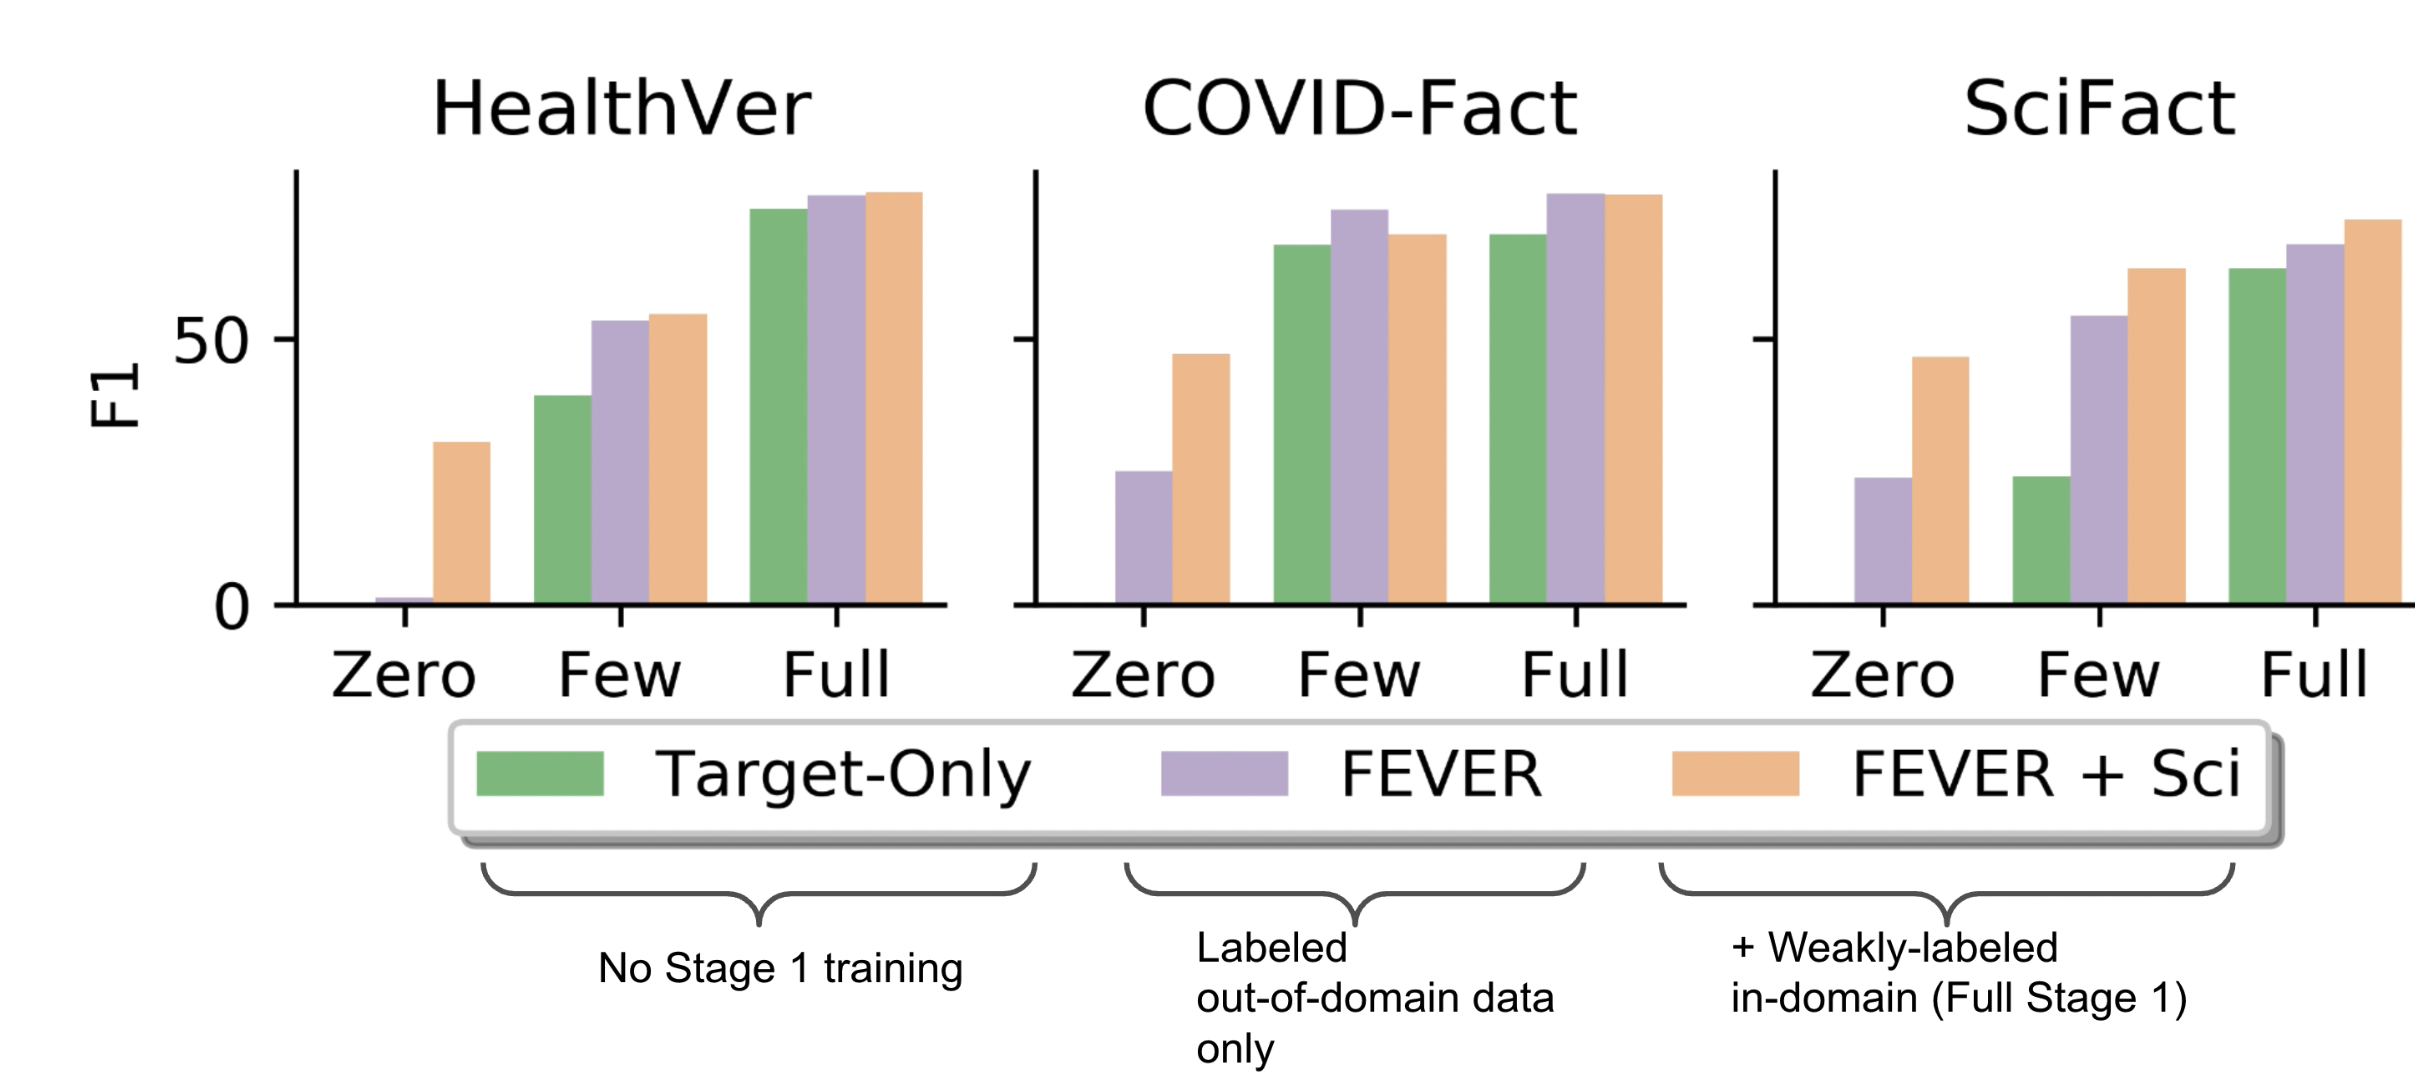
\includegraphics[width=1\textwidth]{Crop/Ablations_3.png}
        }

        \visible<4>{
            \begin{minipage}{0.65\textwidth}
                \begin{block}{}
                    Pretraining with weakly-supervised in-domain data improves few / zero shot performance.
                \end{block}
            \end{minipage}
        }

    
\end{frame}
%------------------------------------------------
 
 


                

\onehalfspacing
\begin{frame} % Use [allowframebreaks] to allow automatic splitting across slides if the content is too long
	\frametitle{Reference}
	
	\begin{thebibliography}{99} % Beamer does not support BibTeX so references must be inserted manually as below, you may need to use multiple columns and/or reduce the font size further if you have many references
		\footnotesize % Reduce the font size in the bibliography
		
		\bibitem[Stanford]{p1}
			\href{https://aclanthology.org/2022.findings-naacl.6}{MULTIVERS: Improving scientific claim verification with
            weak supervision and full-document context}
        \bibitem[Stanford]{p2}
        \href{https://aclanthology.org/2023.findings-acl.387.pdf}{Scientific Fact-Checking: A Survey of Resources and Approaches}
			\newblock Juraj Vladika and Florian Matthes
		
        \hspace{-1.9em}
\includegraphics[width=1.5em]{Icons/github.png}
        \textcolor{blue}{\href{https://github.com/ragavsachdeva/The-Change-You-Want-to-See/tree/main?fbclid=IwAR0LKUHmVIEYSDTCgl2KeV5jir1pUlMSYJTbHbirilqWH_eZ4N9FxHwTQto\#datasets}{Code and model checkpoints for the MultiVerS model}}
          \newblock \textcolor{black}{dwadden/multivers}
	\end{thebibliography}
\end{frame}



%	CLOSING SLIDE
%----------------------------------------------------------------------------------------

\begin{frame} % The optional argument 'plain' hides the headline and footline
	\begin{center}
		{\Huge Thanks for listening!}
		
		\bigskip\bigskip % Vertical whitespace
		
		{\LARGE Q\&A section}
	\end{center}
\end{frame}
%------------------------------------------------


\end{document}
